%
% additional usepackage{beamerthemeshadow} is used
\documentclass{beamer}
\usepackage[utf8]{inputenc}
\usepackage{graphics}
\usepackage{ccicons}
\usepackage[ngerman]{babel}
\usepackage{pdfpages}
%\usepackage{beamerthemeshadow}
\usetheme{Montpellier}
\begin{document}

	\title{Freie Softwareanwendungen\\ geben der Kreativität freien Raum}  
	\author{HG Unckell\hspace{5mm}
	\raisebox{-10mm}{
\includegraphics[height=3cm]{LogoCTB}}
 }
	\date{Juni 2023 - \ccby} 
	
	\frame{\titlepage} 
		\logo{
\includegraphics[height=1.2cm]{LogoCTB}}
	\frame{\frametitle{Übersicht}\scriptsize\tableofcontents} 
	
	\section{Ausgangspunkt - Was ist das Interesse?} 
	\subsection{Anwendungen bestimmen den Nutzen und die Nutzung}
	\frame{ \frametitle{Einstieg}
	Ein persönlicher Computer - PC - (bzw. ein Tablet/Smartphone) gibt Nutzenden neue Möglichkeiten,
	wenn man so will - Freiheitsgrade.\smallskip
	
	Das geschieht über Anwendungen, also Programme, 
	die auf dem jeweiligen Gerät verfügbar sind.
	Sie ermöglichen:
\begin{itemize}\itemsep-0.5mm
	\item Informationen aus dem Internet abzurufen
	\item Email - Kommunikation zu organisieren
	\item Texte zu erstellen und zu drucken
	\item Präsentationen zu erstellen und bzw. zu zeigen
	\item Daten zu organisieren in  Tabelle  (bzw. Datenbank)
	\item Medien abzuspielen / zu bearbeiten (Audio, Video, Bilder)
%	\item Medien
\end{itemize}
%}
%
%\frame{ \frametitle{Das Phänomen der Freien Software}
Der Beginn der PC's, der
persönlichen Computer, liegt
in einer kreativen Szene von Bastlern, die Raum für Kreativität schaffen wollten.
%	
%	\bigskip
%	
%In den vergangenen 40 Jahren 
%gibt es dann unterschiedliche Entwicklungspfade und Ausrichtungen.
%Es gibt Firmen, die sich
%stärker der Marktwirtschaft und deren Zielen verbunden haben.
%Gleichzeitig gilt auch für sie,
%nur was Kunden wirklich nutzt,
%kann auf Dauer am Markt Erfolg haben.
%
%\bigskip
%Es gibt Initiativen, oft als Stiftung organisiert, denen die Zusammenarbeit, das Gemeinwohl, die Selbstwirksamkeit wichtiger sind. Natürlich müssen die Menschen, die sich dort engagieren, auch leben können.
%D.h. auch im Umfeld von freier Software muss es Finanzierungsmodelle geben.
}

	\subsection{Digitale Nachhaltigkeit}

\frame{ \frametitle{Das Thema der Marktkonzentration}
In der digitalen Welt lässt sich viel Geld verdienen. Es geht also auch um Marktmacht und das Thema der digitalen Souveränität
von Nutzenden.
Denn sobald Abhängigkeiten entstehen, die einen Kunden zwingen, den Entwicklungen des Produzenten zu folgen, greift der ,,Lock-in Effekt''.\bigskip

Microsoft ist da, zusammen mit einigen weiteren IT-Konzernen, im Verdacht, seine Marktmacht auszunutzen.\bigskip

Mehr dazu u.a. bei der Begründung des Negativpreises 2023 BigBrotherAward. Dort wird auch auf ein Vorgehen des Bundeskartellamtes hingewiesen. Die Großen der Branche
 haben oft wenig Respekt vor der digitalen Privatsphäre ihrer Nutzenden. 
}

\frame{ \frametitle{Was heißt in diesem Zusammenhang digital nachhaltig?}
Schon im 4. Jahrhundert beschreibt Augustinus von Hippo, 

wie mit nicht-materiellen Gütern umgegangen werden soll: 

sie sollen weitergegeben werden.\smallskip

 Digitale Nachhaltigkeit fragt danach, wie in der heutigen, durch Digitalisierung geprägten Gesellschaft ein ethisch verantworteter Umgang mit digitalen, immateriellen Gütern möglich ist.\smallskip
 
%Was kennzeichnet Digitale Nachhaltigkeit aus?
„Digitale Ressourcen werden dann nachhaltig verwaltet, wenn ihr Nutzen für die Gesellschaft maximiert wird, sodass die digitalen Bedürfnisse gegenwärtiger und zukünftiger Generationen gleichermaßen erfüllt werden.
$\ldots$''\smallskip

Weitere Infos dazu unter \url{https://digitale-nachhaltigkeit.net/}

}
	\subsection{FOSS - freie open source Software}

\frame{ \frametitle{Was bedeutet freie - open source Software?}
Ein Netzwerk, um in diesem Sinn  Software nachhaltig zu gestalten, ist die FSF, die free software foundation. Mehr dazu auf \url{https://fsfe.org}
\\[2mm]

\begin{minipage}{62mm}
	Das ,,frei'' in Freie Software steht für Freiheit, nicht für den Preis. Freie Software garantiert den Nutzenden vier grundlegenden Freiheiten. 
	Ist nur eine dieser Freiheiten nicht gegeben, ist eine Anwendung als proprietär und damit als unfrei anzusehen. 
\end{minipage}%
\begin{minipage}{48mm}\qquad
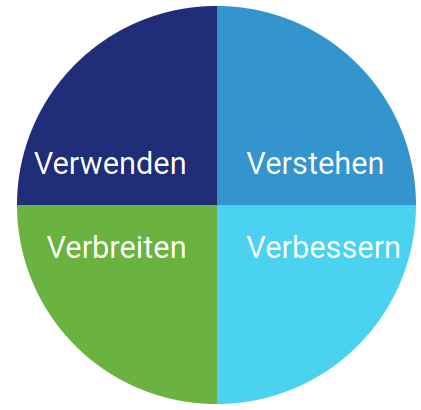
\includegraphics[width=40mm]{Diagramm4F}
\end{minipage}


}%

\frame{\frametitle{Mehr zu den 4 Freiheiten von FOSS }

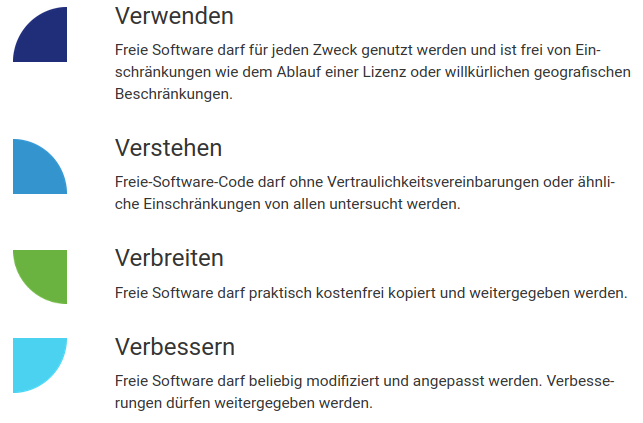
\includegraphics[width=\columnwidth]{4Freiheiten}


}

\frame{\frametitle{Vorteile von FOSS }
\begin{columns}[t]
	\begin{column}{5cm}
\raisebox{-5.3mm}{
\includegraphics[width=15mm]{autonomy}}\quad	Autonomie
	
	\vspace{1mm}	\raisebox{-6mm}{
\includegraphics[width=15mm]{share-copy}}\quad \begin{minipage}{30mm}
			Weitergeben \&\\ Kopieren
		\end{minipage}
	
	\vspace{1mm}\raisebox{-6mm}{
\includegraphics[width=15mm]{reuse}}\quad \begin{minipage}{30mm} Wiederverwenden von Code
	\end{minipage}
	
	\vspace{1mm}\raisebox{-5.3mm}{
\includegraphics[width=15mm]{competition}}\quad Wettbewerb
	\end{column}
	\begin{column}{5cm}
\raisebox{-5.3mm}{
\includegraphics[width=15mm]{collaboration}}\quad		Zusammenarbeit
		
	\vspace{1mm}\raisebox{-5.3mm}{
\includegraphics[width=15mm]{no-lock-in}}\quad	Kein Lock-in Effekt
		
	\vspace{1mm}\raisebox{-5.3mm}{
\includegraphics[width=15mm]{innovation}}\quad	Innovation
		
	\vspace{1mm}\raisebox{-5.3mm}{
\includegraphics[width=15mm]{security}}\quad	Sicherheit
	\end{column}
\end{columns}	
%	\includegraphics[width=\columnwidth]{VorteileFOSS}
	
	
}
	\frame{ \frametitle{Wichtige Eigenschaften der FOSS-Anwendungen}

	Die FOSS-Anwendungen, also Programme, 
	die für das jeweiligen Gerät verfügbar sind,
 kommen aus einer Kultur des Gebens.
 
	D.h. man kann sie nutzen, aber es ist nicht möglich sie zu kaufen.


	
	\bigskip
Sie werden über Initiativen verfügbar gemacht, die oft als Stiftung organisiert sind. \bigskip

So zeigt sich der Wert von Zusammenarbeit und des  Gemeinwohls. 
Außerdem ist die Selbstwirksamkeit der Nutzenden wichtig. 

%Natürlich müssen die Menschen, die sich dort engagieren, auch leben können.
%	D.h. auch im Umfeld von freier Software muss es Finanzierungsmodelle geben.
}


\frame{ \frametitle{Was bedeutet diese Entwicklung für uns?}
FOSS-Anwendungen können oft auf unterschiedlichen Betriebssystemen laufen -
also sowohl auf einem Windows-Rechner, wie einem Apple-Mac oder einem Linuxsystem.
%	Neben Anwendungen, die
%mit dem Betriebssystem mitkommen, gibt es oft freie Anwendungen, die auf unterschiedlichen Systemen laufen und von Stiftungen oder anderen Institutionen stammen.
\bigskip

Wer solche Anwendungen nutzt, vermeidet einen Lock-in Effekt, 
d.h. so einer Person fällt es leichter, bei Bedarf mit den eigenen Daten auf ein anderes System umzuziehen.
\bigskip

Finanzierungsmodelle sind dort anders, ähnlich wie z.B. bei Wikipedia oft auf Spendenbasis,
d.h. für Privatleute meist günstiger.
}
	\section{Freie Software als} 
\subsection{Office-Programme}
\frame{ \frametitle{Libre Office - ein professionelles Anwendungspaket}

Vermutlich nutzen  einige der Anwesenden dieses Paket.

Das Paket enstand aus dem Programm Star Office, 

welches 1985 auf den Markt kam.
\smallskip

LibreOffice erlaubt, Texte, Tabellen, Präsentationen zu erstellen.
Außerdem gibt es Importfilter für Daten, die mit Microsoft-office Programmen erstellt wurden.
\smallskip

Gründe, sich LibreOffice zuzuwenden,
sind u.a. der Respekt vor der digitalen Privatsphäre der Nutzenden.
Microsoft Office wertet nicht transparent Nutzungsdaten aus, so dass Schulen bei uns abgeraten wird, diese Software zu nutzen.
\smallskip

Start mit einem Download von \url{https://www.libreoffice.org/}
	

}

\frame{ \frametitle{Freie Office Versionen sind verfügbar auf  }
	\begin{itemize}
		\item Windows PC
		\item Mac OS
		\item Linux
		\item Online via Browser
		\item Android + iOS
	\end{itemize}
Die Nutzung dieser Versionen ist in über 100 Sprachen möglich
und führt gerade in Ländern der 2. + 3. Welt Menschen an 
diese Möglichkeiten heran ohne die Abhängigkeit von einem kommerziellen 
Quasi-monopolisten.\smallskip

 Das ist dort ein wichtiger Beitrag für das Gemeinwesen. 
}
\subsection{Browser}

\frame{ \frametitle{Firefox -  wichtiger Baustein der Internetnutzung}
	Wie bei vielen anderen FOSS-Anwendungen gehen die Wurzeln von Firefox und Mozilla weit zurück, bis zu Beginn der 90iger.
		
	Start mit einem Download von \url{https://www.mozilla.org}
	\smallskip
	
	
	Die Internet-kommunikation basiert  auf offenen Standards und nachdem sich ein größeres Interesse an diesem Miteinander herauskristallisiert hat, 
	investierte Microsoft stärker in diesen Bereich und die Geschäftsgrundlage alternativer Produkte ging verloren. Deren Code wurde dann zur Grundlage einer Weiterentwicklung, durch die wir nun diese Anwendung haben. 
	\bigskip
	
	
	Firefox ist stärker auf den Datenschutz fokussiert. 
	Auf seiner Grundlage gibt es auch den Email-Client \textbf{Thunderbird}.

	
	Start mit einem Download von \url{https://www.thunderbird.net}
	
	
}

\frame{ \frametitle{Firefox ist verfügbar auf}
	\begin{itemize}
	\item Windows PC
	\item Mac OS
	\item Linux
	\item iOS
	\item Android 
\end{itemize}
	Die Nutzung des Internets ist vermutlich für viele der Hauptgrund, einen PC oder ein Smartphone/Tablet einzuschalten.\bigskip
	
	Je nach Nutzungsverhalten kann daher auch ein altes und somit langsames Gerät noch gute Dienste leisten.
\bigskip

Im Browser lassen sich so auch einige Medien abspielen, Dokumente, wie PDFs anschauen.
}

\subsection{gut zu erweitern für besondere Anwendungsfälle}

\frame{ \frametitle{Freie Anwendungen lassen sich leicht erweitern}

Sowohl für das Libre-Office Paket, wie auch für den Firefox gibt es eine Vielzahl an Add-ons, an Erweiterungen.

So bekommen diese Programme weitere Funktionalität, die den spezielleren Nutzungswünschen entspricht.
\bigskip

Wer also z.B. an Nachrichten stärker interessiert ist, dem könnte  ein Add-on in Firefox zu einem weiteren Internet-standard in diesem Umfeld, dem RSS-feed helfen.
\bigskip

Wer z.B. ab und zu einen fremdsprachigen Text erstellt, der kann von einer Rechtschreibprüfung-Erweiterung im LibreOffice profitieren.
}
\subsection{Option für Mediennutzung}

\frame{ \frametitle{Mediennutzung}

 {\Large VLC media player} \raisebox{-10mm}{
\includegraphics[width=18mm]{VLC_Icon}}
 
 \bigskip
 
VLC ist ein freier und quelloffener Multimediaplayer sowie ein Framework für verschiedene Betriebssysteme, das die meisten Multimediadateien, sowie DVDs, Audio-CDs  und verschiedene Streamingprotokolle abspielt.

\bigskip

Diese Anwendung wird getragen von
VideoLAN,  einer gemeinnützige Organisation \url{https://www.videolan.org}.
}
\subsection{Ausdruckshilfe für Kreativität }
\frame{ \frametitle{Verfügbare Unterstützung für kreatives Arbeiten}
Wenn wir in dieses Umfeld einsteigen, geht es schnell in größere Tiefen, als es für einen solchen Vortrag sinnvoll ist.

Daher nur eine kurze Übersicht zum Abschluss:
\begin{itemize}
	\item 
Bildbearbeitung mit vielen Möglichkeiten bietet z.B. GIMP
\url{https://www.gimp.org/}
\item 
Audiobearbeitung mit vielen Möglichkeiten bietet z.B. Audacity \url{https://www.audacityteam.org/}
\end{itemize}

Achtung, ähnlich wie im Umfeld von VLC media player gibt es auch bei diesen Anwendungen Trittbrettfahrer, die mit ähnlichen Einstiegsnamen im Internet, Nutzenden etwas zur Verfügung stellen, welches 
nicht dem Gewünschten entspricht.
}



\end{document}


